\chapter{Aplicaciones Nativas de la Nube}

\section{Aplicaciones Nativas de la Nube}

    Con el objetivo de encarar los desafíos descritos en el Capítulo 1, el
    uso de tecnologías de computación en la nube a la par de tecnologías de
    composición de servicios es una aproximación utilizada en el mundo del
    desarrollo de software. Tradicionalmente, una aplicación no es
    desarrollada ``orientada a servicios'', ni considerando el uso de
    recursos, ni que esta pueda ``escalar'' de acuerdo a las demandas del
    usuario final. Por lo tanto, a continuación se explican los conceptos de
    computación en la nube, como se relaciona con los llamados servicios y
    que implica un diseño orientado a la nube.

    
	\subsection{Migrando hacia Aplicaciones Nativas de la Nube}
	
    El proceso de reconstruir la arquitectura de una aplicación o servicio para poder utilizar ventajosamente los principios de computación en la nube se conoce como migrar a la nube (en inglés, Cloudification). El resultado de este proceso es una aplicación nativa de la nube (CNA). 
    
    Este tipo de aplicaciones muestran comportamientos y características comunes, pero cabe mencionar que es la arquitectura de la aplicación y no la plataforma destino que la convierten en una aplicación nativa de la nube. De acuerdo con los principios de aplicaciones orientadas a servicios, la arquitectura de una aplicación debe tener bajo acoplamiento y hacer uso de patrones de comunicación asíncronos y sin bloqueo. 
    
    Más aún, es clave para un diseño nativo de la nube exitoso incluir funcionalidades como pooling de recursos, tenencia múltiple, “a pedido” (on-demand) y autoabastecimiento, y principalmente escalabilidad. El último, por ejemplo, se basa en métricas a partir de monitoreo mientras se añaden o eliminan recursos. Cuando estas métricas indican que la demanda aumenta, nuevos recursos son automáticamente añadidos en base a acciones proactivas y/o reactivas. Esto se conoce como escalar hacia fuera. El inverso también existe: cuando la demanda disminuye, los recursos son eliminados, esto se conoce como escalar hacia dentro. Este comportamiento de escalabilidad proporcionan confiabilidad pues la aplicación no percibe ningún tiempo muerto o degradación en la calidad del servicio. De la misma manera, una aplicación nativa de la nube expone actualizaciones sin ninguna percepción de tiempo muerto. 
    
    De manera que las acciones de escalabilidad suceden cuando la aplicación se está ejecutando, surge la oportunidad de realizar optimizaciones tales como reducir el costo al reducir el número de recursos utilizados o el cambio de ubicación de recursos para proporcionar una menor latencia. Una aplicación nativa de la nube debe respetar los principios de computación en la nube que se describen a continuación.
	
        \subsubsection{Principios de la Computación en la Nube}
        El objetivo clave es aprovechar los beneficios que trae una arquitectura nativa de la nube basada en los principios de Computación en la Nube definidos por NIST \parencite{Mell2011-wz}:
        \begin{itemize}
            \item \textbf{Bajo demanda, Autoabastecimiento:} esto significa que los usuarios finales de la nube (de en adelante llamados usuarios finales) pueden ir hacia un proveedor de la nube y, sin ninguna intervención del proveedor de la nube, crear una instancia de un servicio en la nube,  cuando el usuario lo necesite; considerando que los detalles de facturación del usuario final han sido provistos y validados por el proveedor.
            \item \textbf{Pooling de Recursos:} esto significa que los recursos de computación que utiliza un proveedor de servicios en la nube están compartidos a lo largo de las instancias de servicios de los clientes, siguiendo un modelo de Tenencia Múltiple. Utilizando tecnologías de virtualización, el proveedor de servicios en la nube puede utilizar óptima y fácilmente esos recursos. 
            \item \textbf{Acceso de Red Amplio (Broad Network Access):} los servicios en la nube generalmente son entregados a través de la red a través de mecanismos estándar que promueven que el usuario final pueda acceder a los servicios de la nube a través de cualquier plataforma (Laptop, iPad, Smartphone, etc.)
            \item \textbf{Rápida Elasticidad:} esto significa que un usuario final puede fácilmente hacer crecer o encoger sus recursos de computación en base a métricas de desempeño. Esto sucede generalmente añadiendo más instancias de servicios para manejar los cambios en la carga de trabajo (en base a las métricas de desempeño). Es poco frecuente (y no muy recomendado) escalar hacia arriba o hacia abajo la instancia del servicio (por ejemplo, aumentando/disminuyendo los recursos virtuales asignados como CPU o memoria) en base a métricas de desempeño.
            \item \textbf{Servicio Medido / Pago-Sobre-La-Marcha:}  los sistemas de computación en la nube cobran en base a cuantos recursos (almacenamiento, memoria, procesamiento, ancho de banda, etc.) se utiliza a lo largo del tiempo y el proveedor entrega reportes claros de todos los recursos utilizados con su costo asociado. Esto marca principalmente la diferencia entre pagar por un servicio y por un producto.
        \end{itemize}
        
        \subsubsection{Tipos de Servicios}
        En la computación en la nube, los servicios se dividen tradicionalmente en tres tipos:
        \begin{itemize}
            \item \textbf{Infraestructura como Servicio (IaaS):} generalmente servicios de cómputo, almacenamiento y red. Estos ayudan al administrador de sistema/red tradicional entregando infraestructura sobre la cual los desarrolladores de aplicaciones pueden montar sus stacks (pilas) de aplicaciones. SIn embargo, dada la facilidad y practicidad de utilizar estos servicios, los desarrolladores están migrando a roles anteriormente reservados para los administradores. Un movimiento conocido como DevOps envuelve este concepto. Ejemplos de ofertas de infraestructura como servicio son Openstack \footcite{Openstack2016-od}, Amazon EC2 \footcite{Aws2016-fc} and Joyent Triton \footcite{Joyent2016-wr}.
            \item \textbf{Plataforma como Servicio (PaaS): }típicamente conocida como ambientes de ejecución para lenguajes de programación, bases de datos y servidores web. PaaS puede ser visto como un conjunto de servicios que respaldan al programador que quiere entregar su software a usuarios finales. Ejemplos de PaaS son Google AppEngine \footcite{Google2016-zb}, CloudFoundry \footcite{Cloudfoundry2016-vz}, y OpenShift \footcite{RedHat2016-sb}.
            \item \textbf{Software como Servicio (SaaS):} es la categoría más amplia de servicios de computación en la nube, ya que refleja la diversidad que surge de la creatividad de los programadores de aplicaciones y ofrece sus creaciones a los clientes. Ejemplos de estos incluyen Google Apps for Work\footcite{Google2016-ts} and Salesforce \footcite{Salesforce2016-mo}.
        \end{itemize}

        \subsubsection{Principios de una Arquitectura Orientada a Servicios (SOA)}
        
        Un conjunto importante de principios inherentes a la Computación en la Nube es el que indica los lineamientos acerca de las Arquitecturas Orientadas a Servicios (SOA) y, en general, sistemas distribuidos. Estos definen que los servicios sean:
        \begin{itemize}
            \item \textbf{Autónomos: }La lógica de un servicio se encuentra de un límite explícito. El servicio tiene control dentro de sus límites y tiene bajo acoplamiento para la ejecución. 
            \item \textbf{Compartir un contrato formal: }Para que los servicios puedan interactuar, deben compartir únicamente una colección de metadatos públicos que describen a cada servicio y sus términos de intercambio de información.
            \item Bajo acoplamiento: Dependencias entre la lógica subyacente de un servicio y sus consumidores se limitan a las conformidades establecidas en el contrato del servicio. Los servicios abstraen al consumidor de la lógica subyacente, que es invisible al mundo exterior, más allá de lo que está expresado en los metadatos del contrato del servicio.
            \item \textbf{Acoplable (Composable):} Servicios pueden componer servicios, lo que permite que la lógica pueda ser representada con diferentes niveles de granularidad. Esto permite la reusabilidad y la creación de capas de servicios que abstraen y/o plataformas.
            \item \textbf{Reutilizable: }Ya sea que oportunidades inmediatas de reutilización existan, los servicios son diseñados para ser potencialmente re-utilizados.
            Sin estado: los servicios deben ser diseñados para maximizar la falta de estado, aunque esto implique delegar la administración de estado en otro lugar.
            \item \textbf{Reconocible (Discoverable): }Los servicios deben permitir que sus descripciones sean descubiertas y entendidas por (posiblemente) humanos y servicios solicitantes que puedan ser capaces de utilizar su lógica. Los servicios deben ser descubiertos a través de un panorama de servicio
        \end{itemize}
        
        \subsubsection{Entidades Básicas}
        Existen entidades básicas en cualquier arquitectura nativa de la nube o basada en SOA cuya explicación es requerida para poder entender la arquitectura:
        \begin{itemize}
            \item \textbf{Servicio:} OASIS define un servicio como  “un mecanismo capaz de acceder a una o más capacidades, donde el acceso está provisto usando una interfaz prescrita y que es consistente con restricciones y políticas especificadas por la descripción del servicio”. Un servicio puede ser identificado únicamente por su interfaz y su identidad es conocida como su tipo. 
            \item \textbf{Instancia de Servicio (SI):} se define como una única instancia de un servicio de cierto tipo (de servicio).
            \item \textbf{Componente de Instancia de Servicio (SIC):} es un elemento interno e integral de una SI.
            \item \textbf{Recurso:} cualquier componente físico o virtual de disponibilidad limitada dentro de una computadora o sistema de manejo de información. Los recursos de computador incluyen medios para entradas, procesamiento, salida, comunicación y almacenamiento. Un recurso es utilizado por una o más entidades.
            \item \textbf{Recurso Físico:} cualquier elemento de hardware o datos que son parte de un sistema mayor.
            \item \textbf{Recurso Virtual: }un recurso virtual es una fracción temporal y fraccionada de cualquier recurso físico y de disponibilidad limitada en cualquier computador o sistema de manejo de información.
        \end{itemize}
     
        \subsubsection{Microservicios}
        El estilo arquitectónico de “microservicios” \parencite{Lewis2016-az}, inspirado y basado fuertemente en SOA, ha recibido recientemente considerable atención como una solución viable para la construcción de aplicaciones escalables  al utilizar la composición de servicios pequeños, simples, aislados y de funcionalidad única (es decir, microservicios) para construir aplicaciones coherentes. La arquitectura de microservicios va en oposición de la llamada arquitectura “monolítica” donde toda la funcionalidad es ofrecida por una única unidad lógica ejecutable
        \begin{figure}[ht]
            \centering
            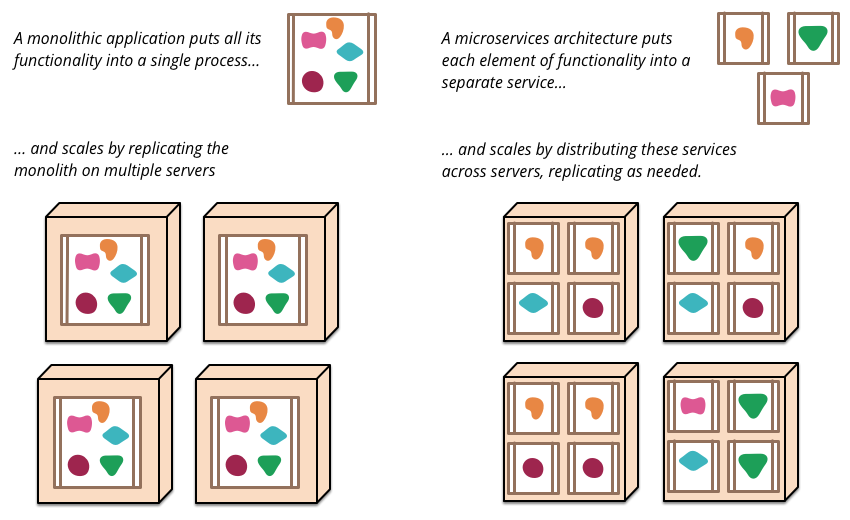
\includegraphics[width=\textwidth]{fowler1}
            \caption{Monolitos y Microservicios (Fowler \& Lewis, 2016)}
            \label{fig:fowler1}
        \end{figure}
    
        {Los principios detrás de una arquitectura de microservicios son:}
        
        \begin{itemize}
            \item {Servicios de bajo acoplamiento con fronteras bien definidas por sus
              interfaces}
            \item {Independencia de Microservicios:}
                \begin{itemize}
                \item {Aislamiento de desempeño y fracasos}
                \item {Delegación a un único equipo}
                \item {Ciclo de entrega propio}
                \item {Mejor tecnología para la tarea}
                \item {Manejo descentralizado de datos }
                \end{itemize}
            \item {Automatización de infraestructura}
            \item {Diseñado para el fracaso}
        \end{itemize} 
        Mientras que la mayoría de los principios surgen de la necesidad de un desarrollo continuo y un proceso de despliegue escalable en términos de los equipos involucrados, reducir dependencias y la necesidad de comunicación entre-equipos, las ventajas técnicas de este estilo arquitectónico son el aislamiento de fracasos y desempeño de manera que las aplicaciones pueden (parcialmente) continuar ejecutándose aún cuando otras funcionalidades no estén disponibles. Las aplicaciones creadas usando el estilo arquitectónico de microservicios adquieren complejidad con múltiples partes movibles que necesitan ser monitoreadas y manejadas, de manera que automatizacion extensiva debe ocurrir.
        \begin{figure}[h]
            \centering
            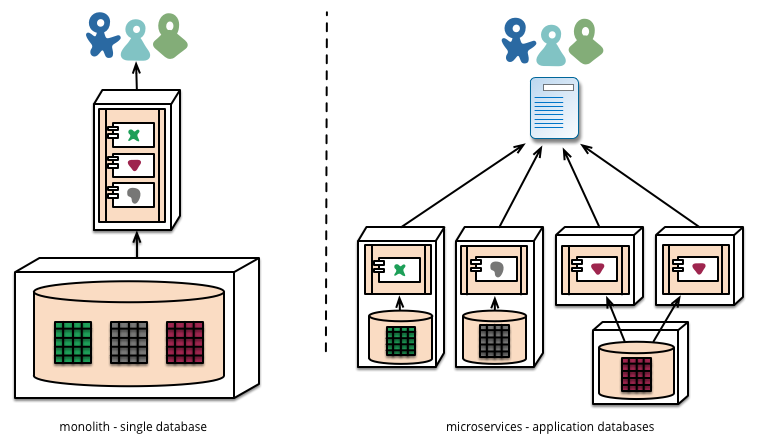
\includegraphics[width=\textwidth]{fowler2}
            \caption{Monolitos y Microservicios \parencite{Lewis2016-az}}
            \label{fig:fowler2}
        \end{figure}

        Los microservicios pueden utilizar diferentes lenguajes de programación y tecnologías de bases de datos en la construcción de una composición coherentes de servicios (modulares). Los microservicios son típicamente provistos y manejados por un proveedor de aplicaciones unico, pero es observable como los mismos principios de gestión necesitados para tratar con composiciones de servicios (que pueden ser de terceros) son necesitadas internamente para las composiciones de microservicios para alcanzar los mismos objetivos generales de confiabilidad.
        
        En las arquitecturas de microservicios, varios patrones pueden ser utilizados para garantizar un comportamiento resistente y de rápida reacción al fracaso. Por ejemplo, el patrón de diseño Circuit-breaker \parencite{Nygard2007-ed} o balanceo de carga (load balancing) en el lado del cliente como en la Netflix Ribbon library \parencite{Netflix2016-ri}. El típico escenario de despliegue tiene múltiples instancias del mismo microservicio ejecutándose simultáneamente, posiblemente con mecanismos de sincronización para servicios con estados. La lógica subyacente es la capacidad de poder instanciar microservicios a lo largo de datacenters y proveedores de infraestructura; permitiendo que cada microservicio se ajuste a los fracasos rápidamente tener puntos de conexión (endpoints) alternativos (para cada tipo de servicio).
        
        De igual manera, los microservicios pueden ser mejorados al seguir buenas prácticas o metodologías a la hora de construir aplicaciones modernas. Una de ellas son los atributos del manifiesto de Los 12 Factores de una Aplicación, que entre otras cosas, enfatiza la importancia de tener un sistema de control de cambios, dependencias explícitas y aisladas, mantener la configuración en el ambiente de desarrollo y no en el código, tratar los servicios de soporte como recursos adjuntos, separar etapas de construcción y de ejecución, ejecutar aplicaciones sin estado y exponer servicios a través la el binding de puertos.

        
    \subsection{Orquestación de Servicios}
        Las arquitecturas orientadas a servicios (SOA) y el estilo arquitectónico de microservicios, como mencionamos, proveen de una manera de construir Sistemas de Tecnologías de la Información (TI) con bajo acoplamiento, alta reusabilidad y utilizando estándares. No obstante, gestionar, configurar y coordinar múltiples servicios complejos manualmente es una tarea que llega a ser tedioso y consume tiempo, y, por lo tanto, dinero. He ahí la necesidad de automatizar estas tareas con la Orquestación de Servicios \parencite{Kapuruge2014-qq}.
        
        La Orquestación de Servicios permite automatizar la configuración y administración de software y las interacciones de software en la nube, las cuales pueden ser eventualmente complicadas cuando sistemas heterogéneos están involucrados y la comunicación se realiza través de diferentes interfaces \footcite{Katsaros2016-bj}. 
        
        En este area han habido iniciativas y trabajos de investigación \parencite{Antonescu2012-ml,Juve2011-ob,Liu2011-vw,Binz2012-ru}, y proyectos en la industria \parencite{Ibm2016-xb,Ibm2013-az} que han utilizado diversas herramientas para la orquestación de aplicaciones en la nube y para describir la topología de servicios.
        
        Una aplicación nativa de la nube generalmente está compuesta por múltiples servicios, cada uno posiblemente compuesto por otros “sub-servicios”, hasta que el "nivel atómico” es alcanzado. Los servicios pueden encontrarse en un datacenter único o dispersos a lo largo de múltiples datacenters (o proveedores) por muchas razones (desde confiabilidad hasta optimización de costos y reducción de latencia para el usuario, segun la zona geográfica del mismo). El objetivo final de la orquestación es costurar (desplegar, provisionar) múltiples componentes para entregar un sistema funcional (por ejemplo, un sistema de bases de datos con replicación) o un servicio (por ejemplo, una aplicación web de 3 capas con API).
	    
	    \subsubsection{Ciclos de Vida}
        En este sentido, cabe mencionar que la orquestación va más allá de la automatización. La automatización es el proceso que permite el abastecimiento y configuración de un nodo individual sin considerar las dependencias que el nodo tenga de otros o viceversa. Aquí es donde la orquestación entra en acción y, junto con la automatización, garantiza el:
        
        \begin{enumerate}
            \item \textbf{Despliegue: }el conjunto completo de recursos y servicios son desplegados según un plan. En esta etapa no son configurados.
            
            \item \textbf{Abastecimiento:} cada recurso y servicio es correctamente abastecido y configurado. Esto debe suceder de manera que se evita que servicio o recurso se encuentre sin una dependencia operacional requerida (por ejemplo, una aplicación PHP sin su base de datos).
        \end{enumerate}

	    El proceso anterior es una abstracción que no incluye las etapas de diseño y ejecución de los componentes orquestados (servicios y/o recursos).
        
        \begin{itemize} 
        \item \textbf{Diseño: }donde la topología y dependencias de cada componente es especificada. El modelo suele representarse con un diagrama o grafo.
        
        \item \textbf{Construcción: }como los artefactos desplegables tales como imagenes de maquinas virtuales (VM), eggs de python, archivos WAR de java son creados a partir de código o recursos existentes. Esto frecuentemente tiene una relación con un proceso de construcción e integración continua.
        
        \item \textbf{Ejecución: }una vez que todos los componentes de una orquestación se están ejecutando, el siguiente paso es gestionarlos. Gestionar significa monitorear los componentes en el nivel más básico. Luego, en base a métricas extraídas, se pueden generar indicadores de desempeño usando reglas lógicas. Finalmente, cuando uno de estos indicadores cruza un umbral preestablecido, un Orquestador puede tomar acciones al respecto.
        
        \item \textbf{Desecho: }de la misma manera que un servicio es desplegado a través de servicios de la nube (por ejemplo, infraestructura a través de VMs), puede que sea necesario destruir la orquestación entera para re-desplegar una nueva versión o solo parte de la orquestación. 
        \end{itemize}

        \subsubsection{Un Ejemplo de Orquestación}
        \begin{figure}[H]
            \centering
            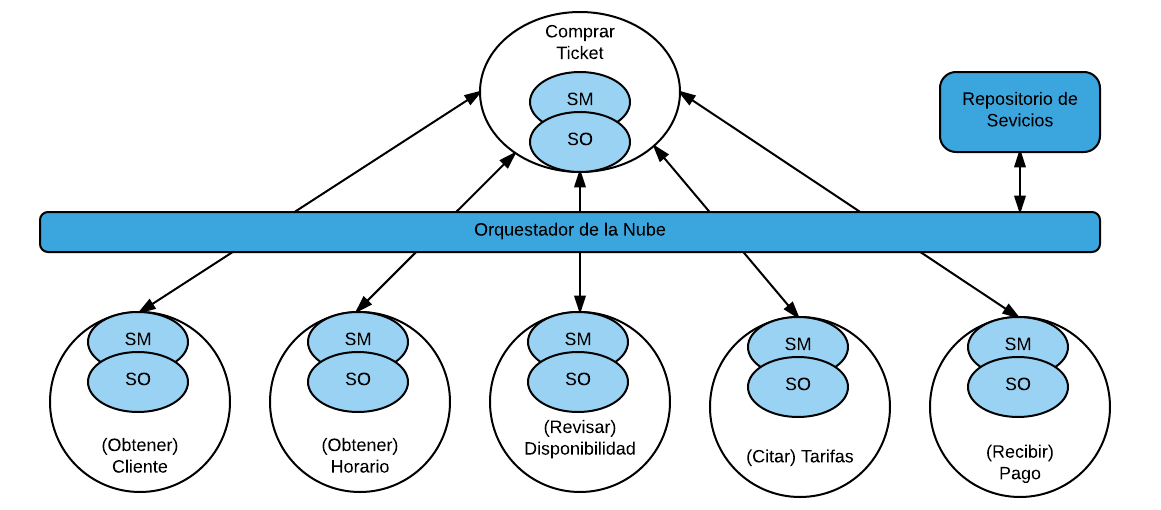
\includegraphics[width=0.90\textwidth]{orch-example}
            \caption{Ejemplo de Servicio Orquestado}
            \label{fig:orch-example}
        \end{figure}
        Por ejemplo, un servicio compuesto, “Comprar Ticket”. Este servicio utiliza las funcionalidades de un conjunto de servicios que son encontrados a través del repositorio de servicios. Estos microservicios, componen el servicio que es entregado y utilizado por el usuario final. 
        
        En el diagrama de la figura \ref{fig:orch-example}, la perspectiva está desde un único cliente o usuario final (tenedor); sin embargo, desde la perspectiva del Orquestador de la Nube, este administra muchas instancias de este servicio. 
        
        La lógica subyacente de coordinar la composición de llamadas entre estos servicios cae bajo el control de la instancia del servicio Comprar Ticket, las cuales son posteriormente ejecutadas por un orquestador.  Este patrón de orquestación hacia abajo se repite para todos los servicios clave, iniciando desde el servicio compuesto. La orquestación de múltiples servicios para combinarlos permite obtener un servicio de extremo a extremo o servicio compuesto. 
        
        En la siguiente sección se describen tecnologías y soluciones clave existentes que pueden realizar la función de orquestación utilizada en contextos de Nubes TI.
	    
	    \subsubsection{Cloudify}
        Cloudify \parencite{Cloudify2016-qi} es una plataforma open-source que provee orquestación de servicios, definiendo la configuración, servicios y dependencias de una aplicación. Utiliza una plantilla YAML, basada en TOSCA, para automatizar el despliegue de una aplicación y describir cómo la aplicación interactúa con el centro de datos a través de APIs.
        
        Cloudify soporta desde la instalación, abastecimiento, configuración y despliegue hasta la gestión y monitoreo de una aplicación o servici
    	    
\begin{figure}[H]
    \centering
    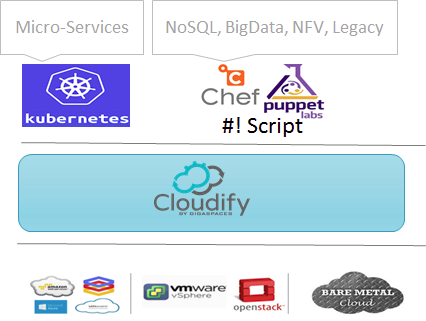
\includegraphics[width=0.75\textwidth]{cloudify-int}
    \caption{Integración de Cloudify \parencite{Cloudify2016-je}}
    \label{fig:cloudify-int}
\end{figure}
    
Características:
\begin{itemize}
\item Orquestación basada en TOSCA.
\item Soporte para gestión y monitoreo de todo el ciclo de vida del servicio
\item Portabilidad de pilas de aplicaciones a cualquier nube o a modelos de nubes híbridas
\item Soporte para cargas de trabajo en contenedores y fuera de contenedores (containerized workloads)
\item Políticas de autocuración y auto-escala
\item Embebible (OEM)
\end{itemize}
Cloudify aporta a la comunidad open-source publicando una de las capacidades principales a través del Proyecto ARIA, que un motor de orquestación basado en las especificaciones TOSCA 
\parencite{Oasis2016-sk}.

\begin{figure}[h]
    \centering
    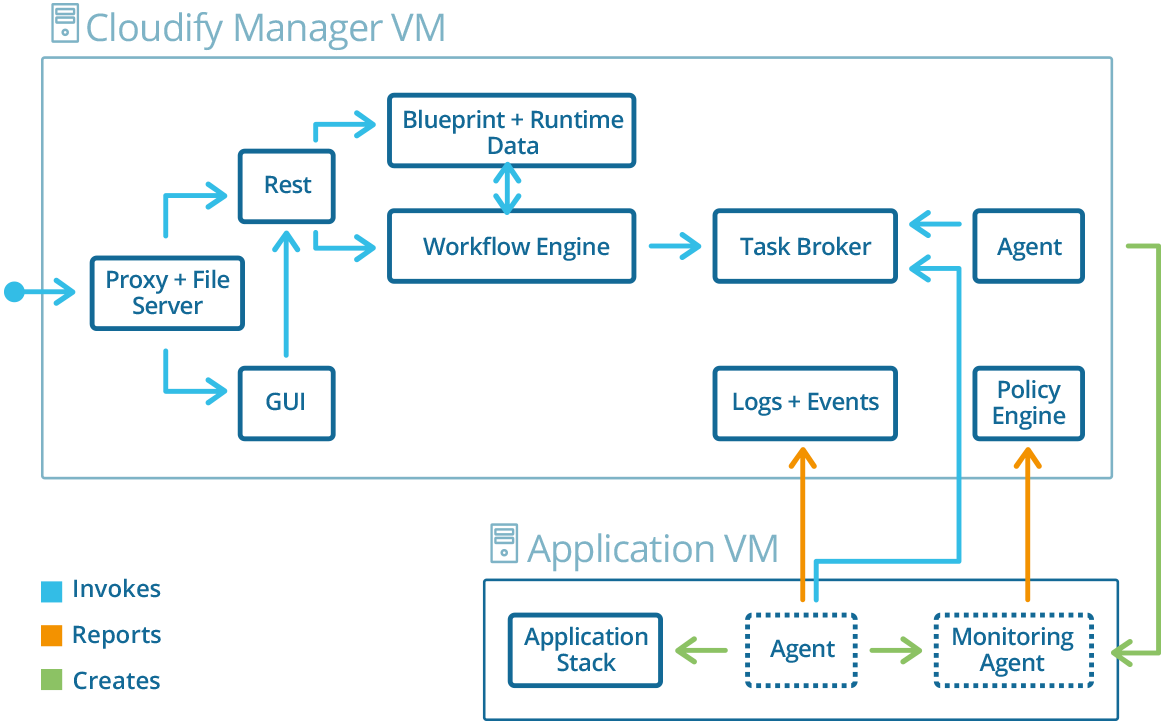
\includegraphics[width=0.80\textwidth]{cloudify-mgr}
    \caption{Resumen de la Arquitectura de  Manager de Cloudify \parencite{Cloudify2016-ze}}
    \label{fig:cloudify-mgr}
\end{figure}

El Manager de Cloudify supervisa el procesamiento de los eventos transmitidos, peticiones seguras, métricas, logs/eventos, ejecución de tareas manuales o automatizadas e interacción con los agentes. Por otro lado, el proxy se encarga de la comunicación con el Manager de Cloudify y los agentes ejecutan tareas en los servidores de aplicaciones (en inglés, application hosts).


\subsubsection{Kubernetes}

Kubernetes es una plataforma open-source para la automatización del despliegue, escalamiento y  operaciones de contenedores de aplicaciones a lo largo de clústeres de servidores (en inglés, clusters of hosts) siendo a la vez ligero y accesible (en inglés, lean), dando soporte para cualquier tipo de nube (portable) y siendo modular, conectable (en inglés, pluggable) y acoplable (en inglés, composable).
Kubernetes soporta preservar el modelo de una aplicación por contenedor, montando sistemas de almacenamiento, distribuyendo secretos, verificando la vida de aplicaciones (en inglés, health-checking), auto-escala horizontal, nombramiento y descubrimiento de servicios, balanceo de carga, monitoreo de recursos, identidad y autorización.
Esto provee la simplicidad de una Plataforma como Servicio (PaaS) con la flexibilidad de una Infraestructura como Servicio (Iaas), y facilita la portabilidad a través de proveedores de infraestructura.

\begin{figure}[H]
    \centering
    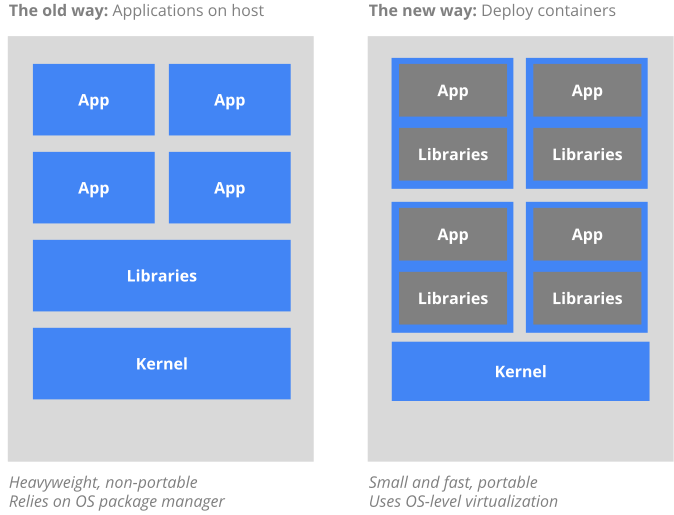
\includegraphics[width=0.80\textwidth]{kub-comp}
    \caption{ Monolitos y Kubernetes \parencite{Kubernetes2016-li}}
    \label{fig:kub-comp}
\end{figure}

Características:
 
\begin{itemize}

\item \textbf{Empaquetamiento Automático: }sin sacrificar disponibilidad, coloca los contenedores automáticamente en base a sus requerimientos de recursos y otras restricciones.
\item \textbf{Autocuración: }reinicia los contenedores que fallan, reemplaza y reprograma (reschedule) a los contenedores cuando un nodo muere; destruye contenedores que no responden a las revisiones de salud (health checks) definidas por el usuario y no los publica a los clientes hasta que estén listos.
\item \textbf{Escalabilidad horizontal}
\item \textbf{Descubrimiento de Servicios y Balanceo de Carga: }soporta el descubrimiento de servicios al dar a cada contenedor una dirección IP y un único nombre DNS para un conjunto de contenedores, y puede realizar balanceo de carga entre ellos.
\item \textbf{Rollouts y Rollbacks Automatizados: }soporta el lanzamiento de cambios a las aplicaciones o a la configuración paulatinamente, mientras monitorea la salud de la aplicación para asegurarse que no se destruyan a todas las instancias de la aplicación al mismo tiempo. Si algo fracasa, Kubernetes ejecuta un rollback del cambio.
\item \textbf{Gestión de secretos y configuración: }soporta el despliegue y la actualización de secretos y la configuración de la aplicación sin reconstruir la imagen y sin exponer los secretos en la configuración del stack.

\end{itemize}

\begin{figure}[H]
    \centering
    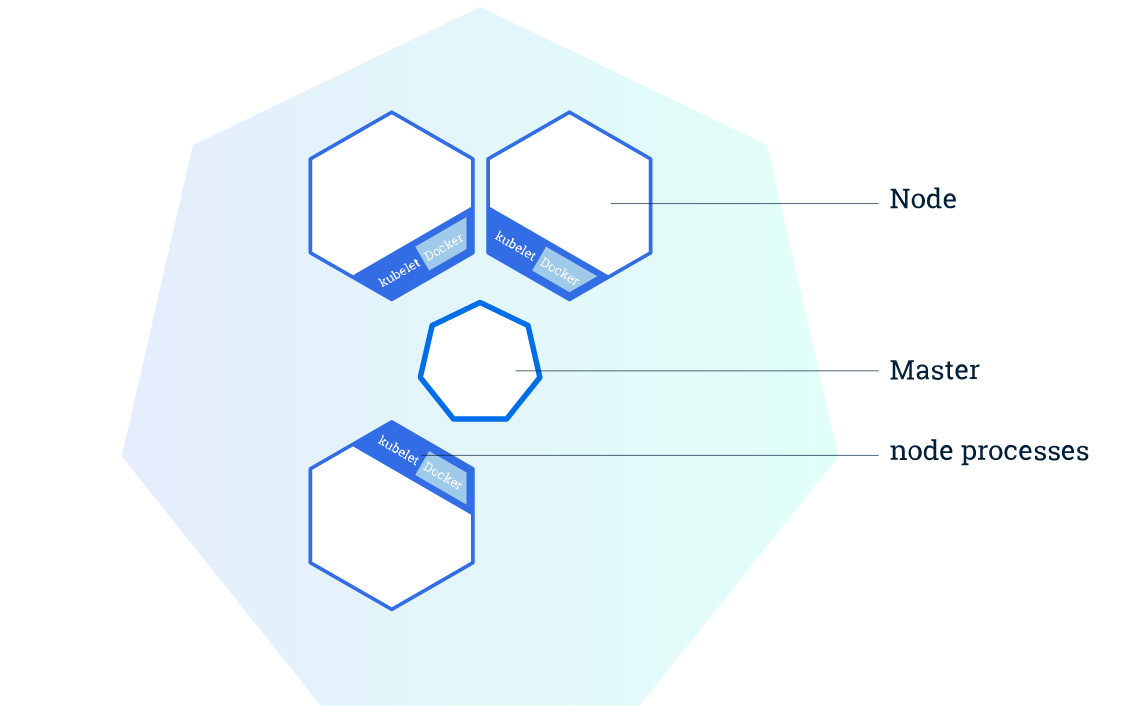
\includegraphics[width=0.80\textwidth]{kub-cluster}
    \caption{ Cluster de Kubernetes \parencite{Kubernetes2016-jo}}
    \label{fig:kub-cluster}
\end{figure}

Un cluster de Kubernetes está compuesto por un nodo maestro que gestiona el cluster y múltiples nodos que hospedan a las aplicaciones que se ejecutan y se comunican con el maestro a través de la API de Kubernetes \parencite{Kubernetes2016-jo}.
consists of a master, which manages the cluster and multiple nodes which host the running applications and communicate with the master through the Kubernetes API.


\subsubsection{Swarm}
Docker Swarm \parencite{Docker2016-yo} es una herramienta de clustering y planificación de contenedores Docker. Provee capacidades nativas de clustering para convertir un conjunto de motores Docker en una sola computadora.

Sus características son:
\begin{itemize}
\item \textbf{Compatible con Herramientas Docker: } soporta la API estándar de Docker, que permite la comunicación con un demonio Docker. También soporta pulling de repositorios privados en DTR  \parencite{Docker2016-is} o Hub \parencite{Docker2016-ev}.
\item \textbf{Alta Escalabilidad y Desempeño: }escala hacia fuera con baja degradación de desempeño. 
\item \textbf{Redes y Volúmenes Integrados: }soporta Redes Docker \parencite{Docker2016-dm}, Volúmenes Docker \parencite{Docker2016-mi} y plugins.
\item \textbf{Alta Disponibilidad y Tolerancia a Fallos: }permite la creación de múltiples maestros Swarm y soporta pólizas para la elección del líder en caso de fallos. También soporta alertas de errores cuando un nodo falla.
\item \textbf{Planificación de Contenedores Flexible: }soporta múltiples filtros tales como etiquetas, afinidad y estrategias para maximizar el desempeño y la utilización de recursos en el momento de asignar contenedores a nodos adyacentes.
\item \textbf{Planificadores y Descubridores de Nodos Conectables: }soporta Mesos o Kubernetes como backend a la par de el cliente Docker. Para el descubrimiento de nodos soporta utilizar un archivo estático, etcd \parencite{Coreos2016-ep}, Consul \parencite{HashiCorp2016-ei} o Zookeper \parencite{Apache2016-oo}.

\end{itemize}

\begin{figure}[H]
    \centering
    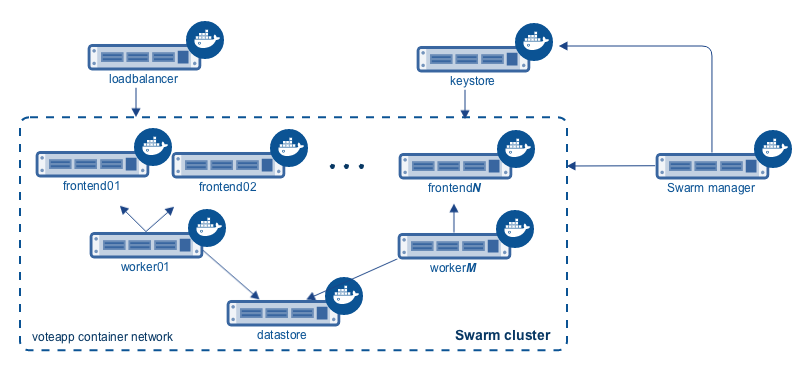
\includegraphics[width=0.80\textwidth]{docker-arch}
    \caption{ Arquitectura de una aplicación Docker \parencite{Docker2016-pk}}
    \label{fig:docker-arch}
\end{figure}
En un cluster Swarm, cada microservicio que compone una aplicación corre dentro de un contenedor Docker y cada uno de los microservicios “Dockerizados” son desplegados en una red de contenedores. Las redes de contenedores son una característica del motor Docker que permite la comunicación de múltiples contenedores a lo largo de múltiples servidores Docker. 

Los cuatro nodos en la Figura X están ejecutando el demonio Docker, al igual que el Manager Swarm y el Load Balancer.


\subsubsection{Juju}
Juju es un orquestador de servicios open-source desarrollado por Canonical Ltd. Se encuentra alojado en Launchpad y bajo la Licencia Pública General Affero (AGPL). Juju separa a los servicios de su contenedor, ya sea el servidor o la máquina virtual en la que son desplegados \parencite{Canonical2016-qx}. 

Juju soporta las siguientes plataformas: Openstack, HP Cloud, Amazon Web Services (AWS), Metal-as-a-Service (MaaS). Ejecutar el procedimiento Juju instancia una máquina virtual  para el Juju State Server, como se muestra en la figura X con la juju-machine-0.


\begin{figure}[H]
    \centering
    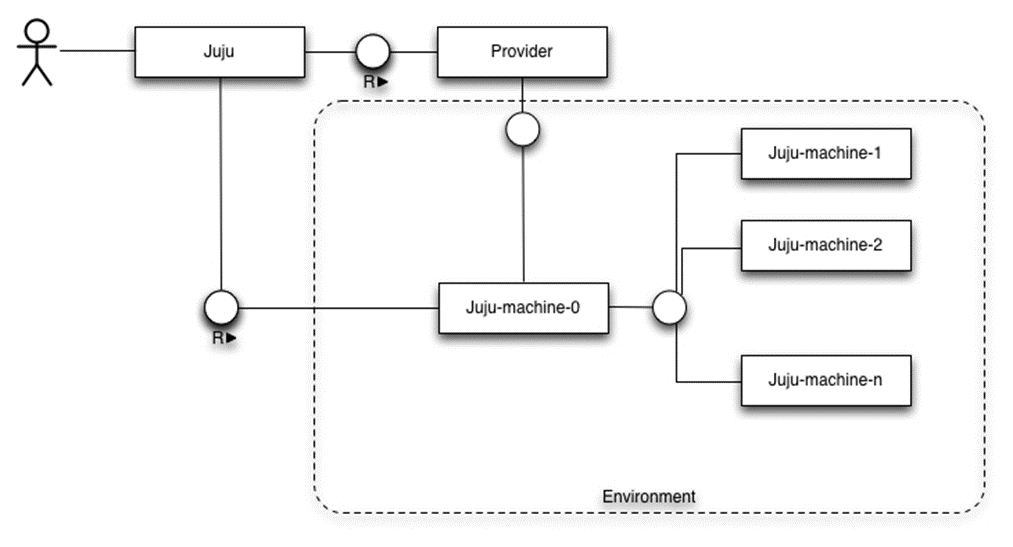
\includegraphics[width=0.80\textwidth]{juju-overview}
    \caption{ Panorama de Juju \parencite{Metsch2013-et}}
    \label{fig:juju-overview}
\end{figure}

Un charm en Juju es el elemento de orquestación de los distintos servicios soportados. En general, para crear un servicio nuevo en Juju es necesario desarrollar y configurar el charm para la gestión del servicio específico. Un charm está definido por sus metadatos y uno o más “ganchos” que son ejecutados a partir del suceso de eventos específicos. 

Los charms de Juju exponen una interfaz que es utilizada por el Juju State Server cuando el usuario envía un comando a través del cliente Juju. 

Juju ofrece también un repositorio de charms donde los desarrolladores pueden desplegar e intercambiar implementaciones de charms. Actualmente existen cientos de charms disponibles que implementan cientos de servicios y herramientas conocidos. Juju proporciona una manera innovadora de orquestar debido a la separación de componentes del núcleo de Juju; esta separación permite introducir nuevos servicios y relaciones sin afectar a componentes clave.


\subsubsection{Heat}

OpenStack Heat es un servicio utilizado para orquestar múltiples aplicaciones nativas de la nube compuestas; utilizando plantillas y a través de una API REST nativa de Openstack y una Interfaz de Programación de Aplicaciones (API) de consultas compatible con CloudFormation \parencite{Rackspace2016-jh}. La figura X muestra un resumen de la arquitectura de OpenStack Heat.
\begin{figure}[h!]
    \centering
    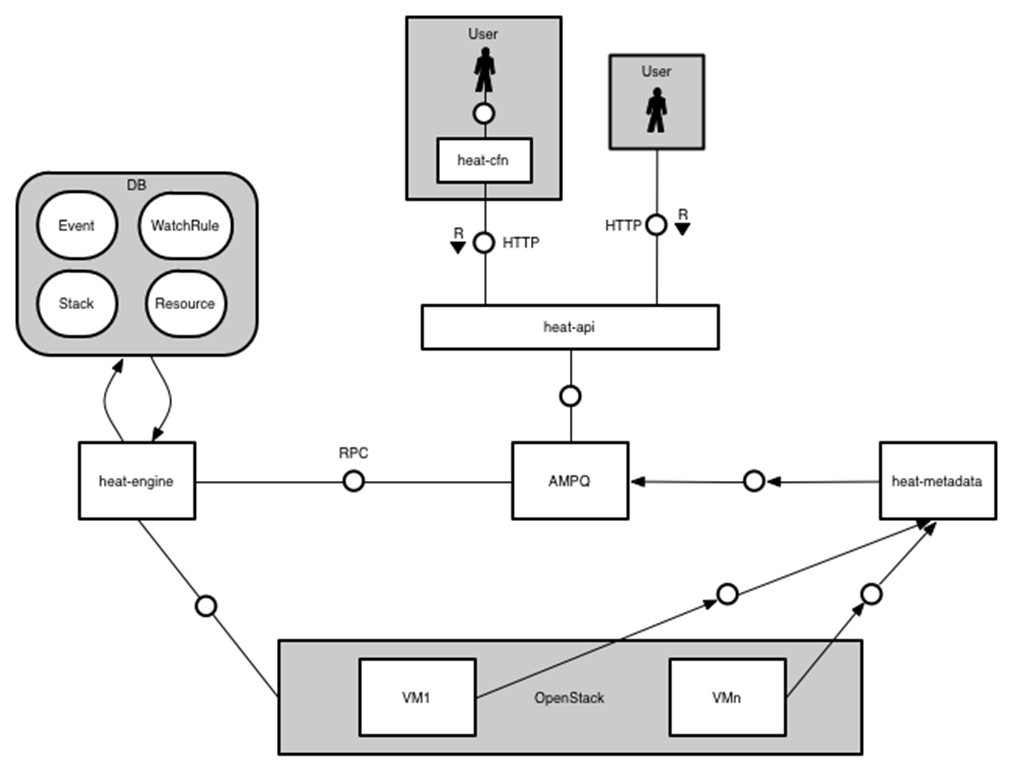
\includegraphics[width=0.80\textwidth]{heat-arch}
    \caption{ Arquitectura de OpenStack Heat \parencite{Metsch2013-et}}
    \label{fig:heat-arch}
\end{figure}
Los componentes principales de OpenStack Heat son:

\begin{itemize}
\item \textbf{Heat:} Heat es una utilidad CLI para OpenStack Heat. Es decir, es una interfaz para agregar, modificar y obtener información acerca de las pilas que pertenecen a un usuario. Es una aplicación de conveniencia que se comunica con el servicio heat-api. heat-cfn utiliza Openstack Keystone para realizar la autenticación antes de comunicarse con el servicio heat-api.
\item \textbf{heat-api:} heat-api es un servicio que expone una API externa basada en REST \parencite{Richardson2008-ng} para conectarse con el servicio heat-engine. La comunicación entre el servicio heat-api y el servicio heat-engine utiliza una cola de mensajes basada en RPC \parencite{Arpaci-Dusseau2015-px}. El servicio heat-api incluye las implementaciones de la API nativa de OpenStack y la API de AWS CloudFormation.
\item \textbf{heat-engine:} la responsabilidad del servicio heat-engine es orquestar el despliegue de plantillas y proveer de eventos a la API del consumidor. Las plantillas se integran bien con herramientas de automatización tales como Puppet \parencite{Puppet2016-ao} o Chef \parencite{Chef2016-cc}.
\item \textbf{heat-metadata:} el servicio heat-metadate recibe metadatos de las pilas de recursos y los guarda en la base de datos.
\item \textbf{AMQP:} broker de mensajes para la comunicación entre servicios.
\item \textbf{Database:} DB subyacente.
\end{itemize}

La funcionalidad básica de Heat funciona cumple con el objetivo de orquestación; no obstante, un problema identificado, aunque mínimo, es la posibilidad de correr comandos init en Heat. Estos comandos init son específicos del sistema operativo y pueden resultar en fallos si la plantilla por un despiste se ejecuta en el sistema operativo equivocado. La solución en este caso es utilizar herramientas de gestión de la configuración como Puppet para asegurar una configuración confiabl

\subsection{Repositorios y Registros de Servicios}
Dados los cambios dinámicos que ocurren en una aproximación basada en servicios (por ejemplo, microservicios), en el momento de enlazar las interfaces de programación de los servicios que se quieren orquestar, debe haber un registro de servicios o un repositorio de servicios que puedan supervisar el descubrimiento y seguimiento de tales servicios.

Un registro de servicios es utilizado en la fase de ejecución para el descubrimiento de servicio, algunas veces y, tradicionalmente a través del estándar UDDI  \parencite{Oasis2016-dc}, interviniendo cuando los servicios desplegados necesitan ser registrados y luego ubicados para ser accedidos por otros servicios. Así pues, se lleva control de las definiciones de servicios, interfaces, parámetros, operaciones, ayudando con la resolución de puntos de conexión y eliminando el “vendor lock-in”.

Por otro lado, un repositorio de servicios, durante todo el ciclo de vida, almacena información acerca del uso de los servicios y aplicaciones que son presentadas en el “catálogo de servicios” y han de ser orquestados. Un repositorio de servicios comúnmente guarda metadatos como la versión, estado, dependencias y responsabilidades, etc. de un servicio.
